\chapter{DESARROLLO DEL PROYECTO}

Este es el capítulo técnico. Recorre la planificación real del proyecto, el \textit{pipeline} implementado y las decisiones que hay detrás, los recursos y el presupuesto, la viabilidad, la sostenibilidad y los resultados obtenidos hasta la fecha.

\section{Planificación del proyecto}

La planificación parte de la estructura en cuatro fases aprobada en el anteproyecto, con una dedicación estimada total de 300~horas. Tras el pivote de diseño documentado en el ADR-004 (véase el apartado de decisiones técnicas), el contenido de cada fase se reformuló en torno al nuevo experimento de robustez de métricas, pero la estructura temporal se mantuvo. La Tabla~\ref{tab:fases} resume las fases, su vinculación con los objetivos específicos (OE) y el esfuerzo asignado.

\begin{table}[H]
  \centering
  \small
  \begin{tabular}{@{}p{0.24\textwidth}p{0.08\textwidth}p{0.46\textwidth}p{0.1\textwidth}@{}}
    \toprule
    \textbf{Fase} & \textbf{OE} & \textbf{Tareas principales} & \textbf{Horas} \\
    \midrule
    Fase~1. Análisis y estado del arte (abril--mayo 2026) & OE1 & Revisión bibliográfica, análisis de Open Specy, selección de \textit{stack}, definición del protocolo de referencia junto con el director & 40 \\
    \addlinespace
    Fase~2. Diseño e implementación (mayo--agosto 2026) & OE1, OE2, OE3 & Reconstrucción del \textit{pipeline} de preprocesado, implementación de las siete métricas, motor de \textit{matching} pandas/Spark, suite de pruebas y CI & 120 \\
    \addlinespace
    Fase~3. Ejecución del experimento y validación (agosto--septiembre 2026) & OE3, OE4, OE5 & Ejecución de la matriz experimental completa con la base de datos de referencia, análisis estadístico, entregable visual & 60 \\
    \addlinespace
    Fase~4. Redacción y cierre (agosto--septiembre 2026) & --- & Redacción de memoria, revisión, defensa & 80 \\
    \bottomrule
  \end{tabular}
  \caption{Fases del proyecto, objetivos específicos asociados y esfuerzo estimado.}
  \label{tab:fases}
\end{table}

A la fecha de esta entrega intermedia (septiembre de 2026), las Fases~1 y~2 están completadas al 100\% y la Fase~3 se ha completado íntegramente, incluida la ejecución del experimento con datos reales: la base de datos de referencia \emph{Hagelskjær Microplastic Solution Library~1.1} se localizó de acceso público (Zenodo, DOI 10.5281/zenodo.17710809, licencia CC-BY-4.0) y se ejecutó la matriz experimental completa (\texttt{scripts/run\_experiment.py --database Databases/Hagelskjaer --full --degradation}), validada numéricamente frente al protocolo de referencia del director (1885 comparaciones alineadas, idéntico al criterio de validación acordado). La Fase~4 avanza con la redacción de los capítulos de resultados, discusión y conclusiones a partir de estos datos reales. La Figura~\ref{fig:gantt} muestra el cronograma y el estado actual.

\begin{figure}[H]
\centering
\begin{tikzpicture}[x=0.9cm, y=0.6cm, font=\small]
% Ejes
\draw[-{Stealth}] (0,0) -- (13,0);
\foreach \m/\lbl in {0.5/Abr, 2.5/May, 4.5/Jun, 6.5/Jul, 8.5/Ago, 10.5/Sep, 12/Oct} {
  \draw (\m,0) -- (\m,-0.15);
  \node[below] at (\m,-0.15) {\lbl};
}
% Barras
\draw[fill=blue!60] (0.5,1) rectangle (3.5,1.6) node[midway,white,font=\tiny\bfseries] {Fase 1};
\draw[fill=blue!60] (2.5,2) rectangle (9,2.6) node[midway,white,font=\tiny\bfseries] {Fase 2};
\draw[fill=orange!70] (7.5,3) rectangle (9.7,3.6) node[midway,white,font=\tiny\bfseries] {Fase 3};
\draw[fill=orange!40] (7,4) rectangle (11,4.6) node[midway,white,font=\tiny\bfseries] {Fase 4};
% Hitos
\draw[red,thick] (1,0.2) -- (1,5) node[above,red,font=\tiny] {Anteproyecto};
\draw[red,thick,dashed] (10,0.2) -- (10,5) node[above,red,font=\tiny] {Entrega intermedia};
\draw[red,thick,dashed] (11,0.2) -- (11,5) node[above,red,font=\tiny] {Entrega final};
% Leyenda
\node[anchor=west] at (0, 5.8) {\footnotesize Azul: fases 1--2 (implementación); Naranja: fases 3--4 (ejecución y redacción)};
\end{tikzpicture}
\caption{Cronograma del proyecto con estado a la entrega intermedia. La Fase~3 se completó, incluida la ejecución del experimento con datos reales, antes de la fecha de esta entrega.}
\label{fig:gantt}
\end{figure}

La memoria se ha ido redactando en paralelo a las Fases~2 y~3, para documentar cada decisión técnica cuando aún estaba fresca y no acumular toda la escritura al final.

\section{Descripción de la solución, metodologías y herramientas empleadas}

\subsection{Visión general del pipeline}

La solución es un paquete Python instalable, \texttt{microraman}, con módulos independientes que se prueban por separado y se encadenan sobre cada espectro medido. La Figura~\ref{fig:pipeline} presenta el flujo de alto nivel, desde la carga del fichero de instrumento hasta el resultado estadístico final.

\begin{figure}[H]
\centering
\begin{tikzpicture}[
  node distance=0.9cm and 1.0cm,
  box/.style={draw, rounded corners=2pt, minimum width=2.5cm, minimum height=0.9cm, align=center, font=\footnotesize},
  src/.style={box, fill=green!20},
  prep/.style={box, fill=blue!20},
  match/.style={box, fill=yellow!30},
  stat/.style={box, fill=red!15},
  arrow/.style={-{Stealth[length=2.5mm]}, thick}
]
\node[src] (io) {Carga\\ (\texttt{io.py}: .wdf)};
\node[prep, right=of io] (crop1) {Recorte\\ por índice};
\node[prep, right=of crop1] (despike) {Despiking\\ (Coca-López)};
\node[prep, below=of despike] (accum) {Acumulación\\ (suma, $N$ niveles)};
\node[prep, left=of accum] (base) {Baseline\\ (airPLS)};
\node[prep, left=of base] (crop2) {Recorte por\\ número de onda};
\node[match, below=of crop2] (metrics) {7 métricas\\ (\texttt{metrics.py})};
\node[match, right=of metrics] (matching) {Matching\\ pandas / Spark};
\node[stat, right=of matching] (stats) {Estadística\\ (Friedman, Wilcoxon)};
\node[stat, right=of stats] (plot) {Entregable\\ visual};
\draw[arrow] (io) -- (crop1);
\draw[arrow] (crop1) -- (despike);
\draw[arrow] (despike) -- (accum);
\draw[arrow] (accum) -- (base);
\draw[arrow] (base) -- (crop2);
\draw[arrow] (crop2) -- (metrics);
\draw[arrow] (metrics) -- (matching);
\draw[arrow] (matching) -- (stats);
\draw[arrow] (stats) -- (plot);
\begin{scope}[on background layer]
  \node[draw, dashed, fit=(crop1) (despike) (accum) (base) (crop2), inner sep=0.3cm, label=below:{\footnotesize\textbf{Preprocesado (\texttt{preprocessing.py} / \texttt{accumulation.py})}}] {};
\end{scope}
\end{tikzpicture}
\caption{Flujo del \textit{pipeline} implementado en el paquete \texttt{microraman}.}
\label{fig:pipeline}
\end{figure}

\subsection{Pipeline de preprocesado}

El preprocesado replica paso a paso el protocolo de referencia acordado con el director del proyecto; el orden es relevante y no se altera sin justificarlo:

\begin{enumerate}
    \item \textbf{Recorte por índice de píxel:} se conservan las columnas \texttt{[220:900]} de la matriz de espectros, descartando los extremos del detector.
    \item \textbf{Eliminación de picos espurios (\textit{despiking}):} método de Coca-López \citep{cocalopez2024despiking} basado en la prominencia y la anchura de los picos (\texttt{scipy.signal.find\_peaks} + \texttt{peak\_widths}); los picos con anchura por debajo de un umbral y prominencia por encima de otro se marcan como espurios y se sustituyen por interpolación lineal a partir de las muestras vecinas no marcadas. El coste sobre el conjunto completo (50.000~espectros) es de aproximadamente 2,4~segundos en un único nodo, por lo que este paso no condiciona el diseño distribuido.
    \item \textbf{Acumulación:} para cada nivel~$N \in \{10000, 5000, 2000, 1000, 500, 200, 100, 50, 20, 10, 5, 2, 1\}$ se calcula la \textit{suma directa} de los primeros~$N$ espectros (no se promedia), simulando un mayor tiempo de integración del instrumento.
    \item \textbf{Corrección de línea base:} se aplica \texttt{airPLS} \citep{zhang2010airpls} (biblioteca \texttt{pybaselines}) al espectro \textit{ya acumulado}, nunca antes de acumular, y se resta la línea base estimada.
    \item \textbf{Recorte final por número de onda:} se restringe a la ventana 2800--3100~cm$^{-1}$ (rango real resultante: 2800{,}51--3099{,}11~cm$^{-1}$).
\end{enumerate}

La equivalencia numérica de esta implementación con el protocolo de referencia del director se comprobó punto a punto sobre los espectros reales mediante el script \texttt{scripts/validate\_vs\_notebook.py}: la diferencia máxima absoluta obtenida es~0.

\subsection{Métricas de similitud espectral}

Se implementan siete métricas en el módulo \texttt{microraman.metrics}, como funciones vectorizables que devuelven siempre una \textit{similitud} (un valor mayor indica mayor parecido), transformando a similitud las que son originalmente distancias:

\begin{itemize}
    \item \textbf{Coseno:} $s_{\cos} = \dfrac{\mathbf{a}\cdot\mathbf{b}}{\lVert\mathbf{a}\rVert\,\lVert\mathbf{b}\rVert}$.
    \item \textbf{Pearson:} correlación lineal entre $\mathbf{a}$ y $\mathbf{b}$ \citep{rodgers1988thirteen}, invariante a desplazamientos aditivos de la línea base.
    \item \textbf{Spearman:} correlación de Pearson calculada sobre los rangos; captura relaciones monótonas no lineales.
    \item \textbf{SAM} (\textit{Spectral Angle Mapper}) \citep{kruse1993sips}: $s_{\text{SAM}} = 1 - \theta/\pi$, con $\theta = \arccos(s_{\cos})$.
    \item \textbf{HQI} (\textit{Hit Quality Index}): $s_{\text{HQI}} = s_{\cos}^{2}$, estándar en librerías comerciales de espectroscopía.
    \item \textbf{Euclídea} y \textbf{Manhattan:} distancias $L_2$ y $L_1$ sobre los vectores normalizados, transformadas a similitud mediante $s = 1/(1+d)$; la normalización previa evita que la métrica dependa de la intensidad absoluta, que crece con la acumulación.
\end{itemize}

\subsection{Protocolo de matching}

El motor de \textit{matching} está implementado por partida doble: \texttt{microraman.matching} (pandas/NumPy, versión de referencia) y \texttt{microraman.matching\_spark} (PySpark), verificadas entre sí sobre datos sintéticos con resultado idéntico. Para cada combinación de polímero medido y nivel de acumulación: (1)~se recorta cada espectro de la base de datos de referencia al rango medido y se descartan los que no solapan lo suficiente; (2)~se interpola el espectro medido al eje de cada espectro de la base de datos por separado, sin extrapolar; (3)~se calcula la similitud con cada métrica y se ordena de forma descendente, conservando el top-4 por combinación.

\subsection{Arquitectura Big Data}

El volumen del problema proviene de la combinatoria polímero $\times$ nivel de acumulación $\times$ métrica $\times$ espectro de la base de datos de referencia, que crece al añadir bases de datos de referencia más amplias. El motor distribuido (\texttt{matching\_spark}) paraleliza el producto polímero~$\times$~nivel sobre los \textit{executors} mediante un \textit{broadcast} de la base de datos completa, de modo que los \textit{executors} no necesitan tener instalado el paquete. El script \texttt{scripts/benchmark\_spark\_scaling.py} mide el \textit{speedup} frente al número de núcleos y frente al motor pandas de un solo nodo; para cargas pequeñas el sobrecoste de Spark domina, y el beneficio de distribuir aparece al escalar el número de espectros de referencia y el número de métricas, lo que delimita cuándo conviene el motor distribuido frente al secuencial.

\subsection{Análisis estadístico}

Se contrasta si existen diferencias significativas entre métricas en su capacidad de identificar el polímero correcto al degradar la calidad del espectro. El diseño es de medidas repetidas: cada bloque es una combinación polímero~$\times$~nivel de calidad, y dentro de cada bloque cada métrica produce un valor. Como variable respuesta se emplea el rango que la métrica asigna al polímero correcto (\texttt{truth\_rank}), independiente de la escala de cada métrica:

\begin{itemize}
    \item \textbf{Contraste ómnibus:} test de Friedman (no paramétrico, medidas repetidas).
    \item \textbf{Tamaño del efecto:} $W$ de Kendall.
    \item \textbf{Post-hoc:} test de Wilcoxon de rangos con signo para cada par de métricas, con corrección de Holm--Bonferroni.
\end{itemize}

Como comprobación de robustez, el mismo análisis se repite sustituyendo la acumulación por una degradación controlada del espectro más limpio de cada polímero (ruido gaussiano a una SNR objetivo, deriva de línea base y submuestreo; módulo \texttt{microraman.degradation}), usando la SNR como eje de calidad independiente. Un ranking de métricas coherente entre ambos mecanismos refuerza la fiabilidad de las conclusiones.

\subsection{Decisiones técnicas y su justificación}

El proyecto pivotó respecto al anteproyecto (ADR-004). La arquitectura inicial, con ingesta mediante Apache Kafka y clasificación con los modelos preentrenados de Open Specy, se sustituyó por la comparación empírica de métricas de similitud frente a la degradación de calidad. El director y yo acordamos el cambio por dos razones: la pregunta nueva no estaba respondida en la literatura, y era abordable con los datos reales disponibles. La Tabla~\ref{tab:decisiones} sintetiza las decisiones vigentes y su justificación.

\begin{table}[H]
  \centering
  \small
  \begin{tabular}{@{}p{0.22\textwidth}p{0.22\textwidth}p{0.46\textwidth}@{}}
    \toprule
    \textbf{Decisión} & \textbf{Alternativas consideradas} & \textbf{Justificación} \\
    \midrule
    Motor distribuido: Apache Spark (PySpark) & Dask, Ray & Madurez y ecosistema; API de DataFrame/RDD adecuada para paralelizar por bloques independientes (polímero~$\times$~nivel) \citep{zaharia2010spark, zaharia2016spark, armbrust2015sparksql}. \\
    \addlinespace
    Diseño experimental: robustez de métricas frente a degradación (pivote ADR-004) & Clasificador entrenado envolviendo Open Specy & Mayor valor científico al no existir una comparación sistemática publicada; evita depender de modelos preentrenados sobre un dominio (microplásticos) para el que no fueron ajustados. \\
    \addlinespace
    Corrección de línea base: airPLS (\texttt{pybaselines}), tras acumular & IModPolyFit, corrección antes de acumular & Coincide con el protocolo de referencia validado con el director; aplicarla antes de acumular distorsiona la suma. \\
    \addlinespace
    Verificación cruzada pandas/Spark & Confiar únicamente en la implementación distribuida & Permite detectar errores de paralelización comparando resultados idénticos sobre el mismo dato sintético antes de ejecutar con datos reales. \\
    \addlinespace
    Empaquetado como librería instalable (\texttt{pyproject.toml}) + CI (GitHub Actions) & Scripts sueltos sin empaquetar & Reproducibilidad, facilita los 97 tests automatizados y evita regresiones al iterar el pipeline. \\
    \bottomrule
  \end{tabular}
  \caption{Decisiones técnicas clave del proyecto, tras el pivote de diseño (ADR-004), y su justificación.}
  \label{tab:decisiones}
\end{table}

\subsection{Metodología de trabajo}

El proyecto adopta una metodología iterativa e incremental con entregables verificables por tarea (un módulo del \textit{pipeline}, un conjunto de pruebas, un script de validación, etc.). Las reuniones periódicas con el director del proyecto, D.~Nico Coca López, sirven como control de avances, validación de decisiones técnicas y punto de origen del pivote de diseño (ADR-004), documentado en el acta correspondiente. El código se versiona en un repositorio Git privado (\texttt{github.com/Lavishmxgames/master\_bigdata}), con integración continua mediante GitHub Actions que ejecuta la suite de pruebas y el análisis de estilo (\texttt{ruff}) en cada cambio. La memoria del TFM se gestiona en un repositorio Git independiente, separado del código (véase el Anexo~C para la URL completa), y se redacta en paralelo al desarrollo para reflejar con fidelidad las decisiones tomadas.

\subsection{Datos del proyecto}

La solución se valida con dos niveles de datos complementarios:

\begin{itemize}
    \item \textbf{Datos reales:} 5~polímeros (PET, PP, PLA, BioPBS y ECOVIO), con 10.000~espectros Raman de integración corta por polímero en la región C--H ($\sim$2900~cm$^{-1}$), medidos en un equipo Renishaw (ficheros \texttt{.wdf}) y proporcionados por el director del proyecto. Cada espectro está etiquetado con su polímero real.
    \item \textbf{Base de datos de referencia:} el experimento emplea la \emph{Hagelskjær Microplastic Solution Library~1.1} \citep{hagelskjaer2025library} (30~espectros de referencia: 28~polímeros y 2~minerales, formato de texto plano). No fue proporcionada por el director del proyecto, sino localizada de acceso público en Zenodo (DOI 10.5281/zenodo.17710809, licencia CC-BY-4.0) a partir de una indicación del propio director de que la biblioteca era de acceso público. Se descartó 1~espectro por solape insuficiente con la ventana medida (2800--3100~cm$^{-1}$), quedando 29~espectros de referencia útiles.
\end{itemize}

\section{Recursos requeridos}

Los recursos utilizados en el proyecto se agrupan en técnicos, humanos y de información:

\begin{itemize}
    \item \textbf{Técnicos:} equipo de desarrollo personal; entorno Python~3.11 con \textit{stack} \textit{open-source} (NumPy, SciPy, pandas, PySpark, \texttt{pybaselines}, \texttt{renishawWiRE}, \texttt{ramanchada2}, pytest, ruff, Git); integración continua con GitHub Actions; editor LaTeX para la redacción de la memoria; gestor bibliográfico (Zotero).
    \item \textbf{Humanos:} autor del TFM (Jesús Baeza Anguiano) como responsable técnico y de redacción; director del proyecto (Nico Coca López) como supervisor científico, autor del protocolo de referencia y aportador de los espectros medidos; la base de datos de referencia empleada para el \textit{matching} se localizó de acceso público (véase el apartado «Datos del proyecto»).
    \item \textbf{Información:} notebook de referencia del director del proyecto para la validación del \textit{pipeline}; artículos científicos accesibles a través del portal bibliográfico de la Universidad Europea de Madrid.
\end{itemize}

\section{Presupuesto}

La Tabla~\ref{tab:costes} presenta la estimación económica del proyecto. El proyecto es viable en términos económicos gracias al uso exclusivo de tecnologías \textit{open-source} y al hardware personal disponible; el coste efectivo desembolsado es nulo, y el presupuesto recoge una valoración de equivalencia en mercado.

\begin{table}[H]
  \centering
  \small
  \begin{tabular}{@{}p{0.3\textwidth}p{0.2\textwidth}p{0.4\textwidth}@{}}
    \toprule
    \textbf{Tipo de coste} & \textbf{Valor estimado} & \textbf{Comentarios} \\
    \midrule
    Horas de trabajo del autor & 300~h ($\sim$9.000~\euro) & Estimación a tarifa de ingeniero de datos júnior (30~\euro/h). \\
    \addlinespace
    Supervisión (director) & 20~h ($\sim$1.500~\euro) & Estimación a tarifa de consultor (75~\euro/h). \\
    \addlinespace
    Equipo técnico & 1.200~\euro{} & Portátil propio del autor, valor de mercado aproximado. \\
    \addlinespace
    \textit{Software} & 0~\euro{} & Todo el \textit{stack} es \textit{open-source}. \\
    \addlinespace
    Acceso a bibliografía & 0~\euro{} & Cubierto por la suscripción de la Universidad Europea. \\
    \addlinespace
    Materiales y \textit{datasets} & 0~\euro{} & Espectros Raman aportados por el director; base de datos de referencia de acceso público (Zenodo, CC-BY-4.0). \\
    \midrule
    \textbf{Total (equivalencia mercado)} & \textbf{$\sim$11.700~\euro} & Desembolso efectivo: 0~\euro. \\
    \bottomrule
  \end{tabular}
  \caption{Estimación del presupuesto del proyecto.}
  \label{tab:costes}
\end{table}

\section{Viabilidad}

Viabilidad técnica, temporal y económica:

\begin{itemize}
    \item \textbf{Viabilidad técnica:} el \textit{pipeline} de preprocesado, las siete métricas y el motor de \textit{matching} (pandas y Spark) están implementados, probados y validados numéricamente frente al protocolo de referencia. El riesgo técnico residual es bajo: no depende de tecnología inmadura, sino de la disponibilidad de un dato externo (la base de datos de referencia).
    \item \textbf{Viabilidad temporal:} el riesgo más relevante identificado durante el proyecto era la dependencia de la base de datos de referencia. Se mitigó localizándola de acceso público y ejecutando el experimento completo antes de esta entrega intermedia (7~sep). Queda así todo el margen hasta el depósito final para pulir Resultados, Discusión y Conclusiones sobre las cifras ya obtenidas.
    \item \textbf{Viabilidad económica y sostenibilidad:} el coste efectivo es nulo, y la solución, al basarse en tecnologías \textit{open-source} ampliamente adoptadas y en un paquete instalable con pruebas automatizadas, tiene un bajo coste de mantenimiento y puede reutilizarse con otras bases de datos de referencia sin rediseñar el \textit{pipeline}.
\end{itemize}

\section{Sostenibilidad del proyecto}

La sostenibilidad se entiende aquí en sus tres dimensiones habituales: la ambiental, referida al efecto sobre los ecosistemas y sobre el consumo de recursos; la social, referida al acceso al conocimiento y a la salud de las poblaciones afectadas; y la económica, referida al coste de operación y a la reutilización de lo construido. El proyecto se sitúa de lleno en la primera y toca las otras dos de forma indirecta.

\subsection*{Dimensión ambiental}

El objeto de estudio es, en sí mismo, un problema ambiental. La identificación fiable de microplásticos es el paso previo a cualquier política de vigilancia o de mitigación: no se puede regular lo que no se sabe medir. El proyecto contribuye a los Objetivos de Desarrollo Sostenible de la Agenda 2030 de Naciones Unidas por dos vías. De forma directa al ODS~14 (\emph{Vida submarina}), cuya meta 14.1 persigue reducir de forma significativa la contaminación marina, incluida la procedente de detritos plásticos; e indirectamente al ODS~6 (\emph{Agua limpia y saneamiento}) y al ODS~12 (\emph{Producción y consumo responsables}), que dependen de poder cuantificar la presencia de estos materiales en el medio.

Hay además un efecto ambiental derivado del propio método. Determinar qué métrica de similitud tolera mejor los espectros de integración corta permite acortar el tiempo de medida por partícula sin perder fiabilidad en la identificación. Un menor tiempo de integración se traduce en menos horas de instrumento por muestra, y por tanto en menor consumo energético del equipo Raman y mayor número de partículas analizadas con los mismos recursos.

\subsection*{Dimensión social}

La contaminación por microplásticos es también un asunto de salud pública, lo que conecta el trabajo con el ODS~3 (\emph{Salud y bienestar}). Más allá del objeto de estudio, el enfoque adoptado tiene una consecuencia social concreta: reducir el tiempo de instrumento por muestra abarata el análisis y lo hace accesible a laboratorios con menos recursos, que son precisamente los de muchas de las regiones más expuestas a esta contaminación. En la misma línea, el proyecto se apoya en una biblioteca espectral de acceso público y publica su propio código, en coherencia con las prácticas de ciencia abierta.

\subsection*{Dimensión económica}

El coste efectivo del proyecto es nulo, al estar construido íntegramente sobre tecnologías \textit{open-source} y hardware ya disponible (véase el apartado de presupuesto). El diseño como paquete instalable, con pruebas automatizadas e integración continua, mantiene bajo el coste de mantenimiento y permite reaprovechar el trabajo con otras bibliotecas de referencia sin rediseñar el \textit{pipeline}.

\subsection*{Estrategias adoptadas}

De este análisis se derivan cuatro decisiones que el proyecto ya aplica y que conviene mantener en su continuación:

\begin{enumerate}
    \item Publicar el código como paquete abierto y reutilizable, en lugar de como scripts de un solo uso, para que el esfuerzo invertido sirva a otros grupos.
    \item Emplear bibliotecas espectrales de acceso público en vez de generar mediciones nuevas cuando ya existen, evitando duplicar consumo de instrumento.
    \item Orientar el resultado del experimento hacia la recomendación práctica de qué métrica usar con tiempos de integración cortos, que es la vía por la que el trabajo puede reducir el gasto energético del análisis.
    \item Documentar el procedimiento de forma reproducible, condición para que los resultados puedan verificarse y reutilizarse sin repetir el trabajo experimental.
\end{enumerate}

\section{Resultados parciales del proyecto}

A la fecha de esta entrega intermedia se han alcanzado los siguientes hitos técnicos, cada uno vinculado con su objetivo específico. A diferencia de la planificación original, la Fase~3 se completó íntegramente, por lo que esta sección ya incluye resultados obtenidos con la base de datos de referencia real (no sintética):

\begin{itemize}
    \item \textbf{OE1 completado:} el \textit{pipeline} de preprocesado (recorte por índice, \textit{despiking} de Coca-López, acumulación por suma, corrección de línea base airPLS, recorte final por número de onda) está implementado en el módulo \texttt{microraman} y validado punto a punto frente al protocolo de referencia del director sobre los espectros reales, con una diferencia máxima absoluta de~0 (\texttt{scripts/validate\_vs\_notebook.py}).
    \item \textbf{OE2 completado:} las siete métricas de similitud (coseno, Pearson, Spearman, SAM, HQI, euclídea, Manhattan) están implementadas como funciones vectorizables con una convención homogénea de similitud, y cubiertas por pruebas unitarias.
    \item \textbf{OE3 completado, incluida la ejecución con datos reales:} la matriz experimental (polímero~$\times$~nivel de acumulación~$\times$~métrica~$\times$~espectro de referencia) se ejecutó sobre la base de datos de referencia real Hagelskjær (paralelización con PySpark disponible y verificada, aunque no necesaria a esta escala: 13195~filas en el eje de acumulación y 8120 en el de degradación, resueltas en segundos con el motor pandas). La validación numérica frente al protocolo del director se superó: \textbf{1885 comparaciones alineadas} (5~polímeros~$\times$~13~niveles~$\times$~29~espectros de referencia), idéntico al criterio acordado.
    \item \textbf{OE4 completado, con resultado real:} test de Friedman sobre el rango asignado al polímero correcto (\texttt{truth\_rank}), restringido a los tres polímeros con verdad-terreno presente en la base de datos de referencia (véase la limitación señalada más abajo). Acumulación real: $\chi^2=8{,}70$, $p=0{,}191$, $W$ de Kendall $=0{,}037$ (0/21 pares significativos tras corrección de Holm). Degradación paramétrica: $\chi^2=19{,}35$, $p=0{,}0036$, $W=0{,}134$ (también 0/21 pares individuales significativos tras Holm).
    \item \textbf{OE5 completado:} el entregable visual solicitado por el director (similitud del mejor resultado frente al nivel de acumulación, una curva por métrica y por polímero) se generó con datos reales; véase la Figura~\ref{fig:similitud-acumulacion}.
\end{itemize}

El proyecto cuenta con 97~pruebas automatizadas en verde, ejecutadas en integración continua (GitHub Actions) en cada cambio, un paquete instalable (\texttt{pip install -e .}) y un repositorio Git separado para el código (\texttt{master\_bigdata}) y otro, independiente, para esta memoria (véase el Anexo~C). El experimento completo se ejecutó y validó antes de esta entrega intermedia.

\subsection{Resultados obtenidos}

La Tabla~\ref{tab:accuracy} resume la exactitud de cada métrica en la identificación del polímero correcto (rango~1 y entre los tres primeros), restringida a los tres polímeros con verdad-terreno presente en la base de datos de referencia (PET, PLA, PP):

\begin{table}[H]
  \centering
  \small
  \begin{tabular}{@{}lp{0.24\textwidth}p{0.1\textwidth}p{0.1\textwidth}p{0.12\textwidth}@{}}
    \toprule
    \textbf{Eje de calidad} & \textbf{Métrica} & \textbf{Acc.@1} & \textbf{Acc.@3} & \textbf{Rango medio} \\
    \midrule
    Acumulación real & Pearson & 61,5\% & 79,5\% & 3,26 \\
    Acumulación real & Coseno = Euclídea = HQI = SAM & 53,8\% & 74,4\% & 4,36 \\
    Acumulación real & Manhattan & 41,0\% & 56,4\% & 4,28 \\
    Acumulación real & Spearman & 41,0\% & 69,2\% & 4,59 \\
    \addlinespace
    Degradación paramétrica & Coseno = Euclídea = HQI = SAM & 87,5\% & 95,8\% & 1,25 \\
    Degradación paramétrica & Pearson & 83,3\% & 100\% & 1,21 \\
    Degradación paramétrica & Manhattan & 70,8\% & 87,5\% & 1,63 \\
    Degradación paramétrica & Spearman & 54,2\% & 100\% & 1,75 \\
    \bottomrule
  \end{tabular}
  \caption{Exactitud de cada métrica de similitud (PET/PLA/PP), por eje de degradación de calidad.}
  \label{tab:accuracy}
\end{table}

El orden cambia según el eje. Con acumulación real gana Pearson; con degradación paramétrica, el grupo coseno, euclídea, HQI y SAM, que empata en las cuatro. Ninguna diferencia entre métricas es, sin embargo, significativa por pares tras la corrección de Holm (véase OE4). Léanse por tanto como tendencia y no como superioridad demostrada: solo tres polímeros tienen verdad-terreno disponible.

\begin{figure}[H]
\centering
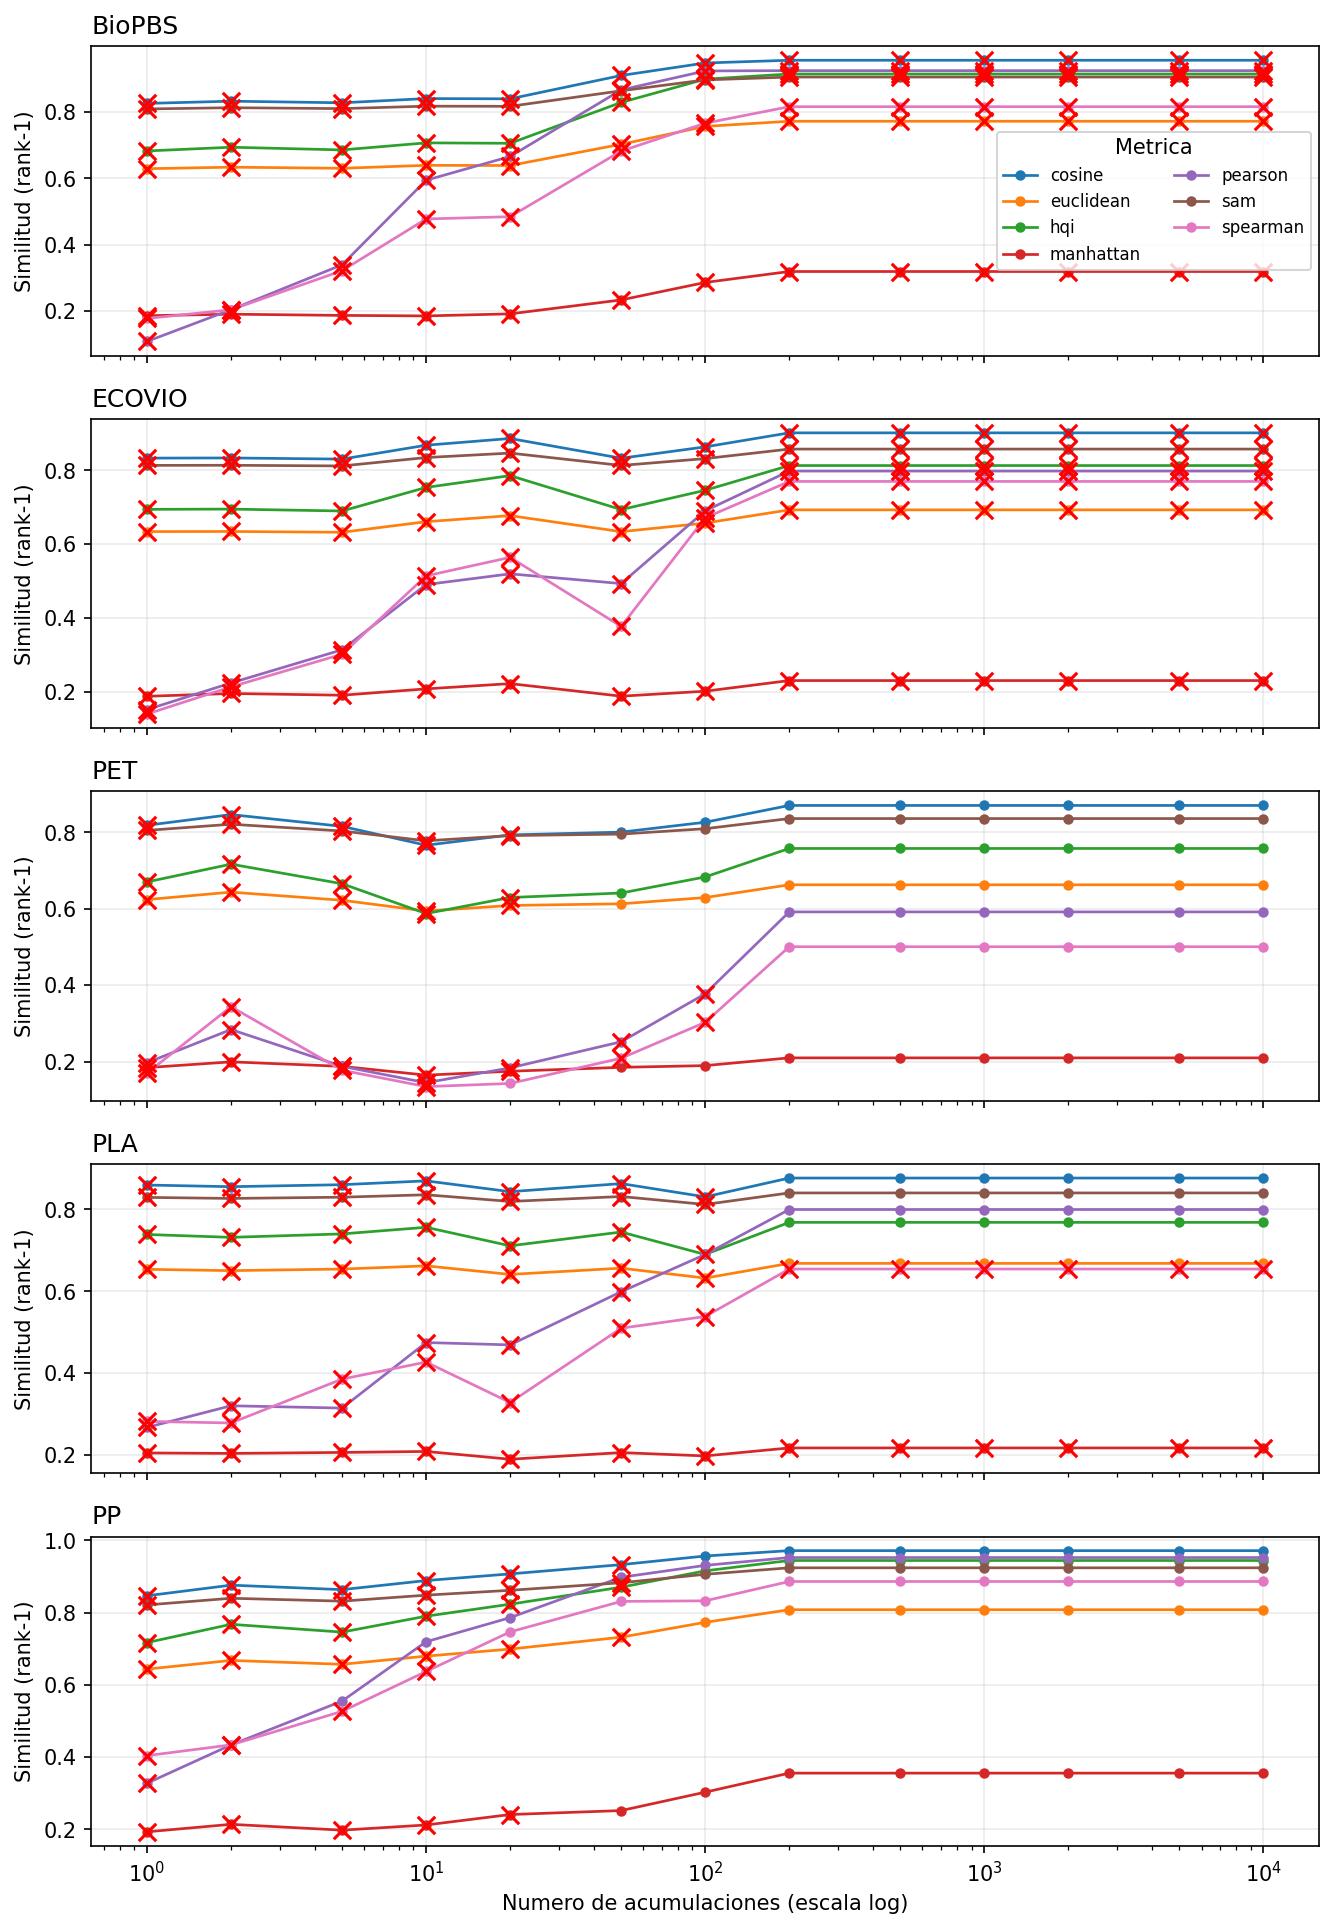
\includegraphics[width=0.85\textwidth]{imagenes/accumulation_similarity.png}
\caption{Similitud del mejor resultado (rango~1) frente al número de acumulaciones, una curva por métrica, una subgráfica por polímero medido. La cruz roja marca el punto en que el rango~1 deja de ser el polímero correcto.}
\label{fig:similitud-acumulacion}
\end{figure}

\textbf{Punto de ruptura y ranking de robustez.} El punto de ruptura de una métrica para un polímero es el nivel de calidad mínimo a partir del cual el resultado de rango~1 es el polímero correcto \emph{de forma estable} (es decir, también para todos los niveles superiores). La Tabla~\ref{tab:ruptura} lo agrega por métrica y la Figura~\ref{fig:heatmap-acumulacion} lo desglosa por polímero.

\begin{table}[H]
  \centering
  \small
  \begin{tabular}{@{}p{0.2\textwidth}p{0.26\textwidth}p{0.13\textwidth}p{0.1\textwidth}p{0.14\textwidth}@{}}
    \toprule
    \textbf{Eje de calidad} & \textbf{Métrica} & \textbf{Ruptura media} & \textbf{Mediana} & \textbf{Polímeros nunca identificados} \\
    \midrule
    Acumulación ($N$) & Pearson & 101,7 & 100 & 2 \\
    Acumulación ($N$) & Coseno = Euclídea = HQI = SAM & 116,7 & 100 & 2 \\
    Acumulación ($N$) & Spearman & 110,0 & 110 & 3 \\
    Acumulación ($N$) & Manhattan & 50,0 & 50 & 3 \\
    \addlinespace
    Degradación (SNR) & Coseno = Euclídea = HQI = SAM & 2,7 & 2,0 & 2 \\
    Degradación (SNR) & Pearson & 3,7 & 5,0 & 2 \\
    Degradación (SNR) & Spearman & 3,5 & 3,5 & 3 \\
    Degradación (SNR) & Manhattan & 1,0 & 1,0 & 3 \\
    \bottomrule
  \end{tabular}
  \caption{Punto de ruptura por métrica y eje de degradación de calidad. Un valor menor indica que la métrica tolera más degradación antes de fallar; la última columna indica sobre cuántos de los cinco polímeros medidos la métrica no llega a acertar en ningún nivel.}
  \label{tab:ruptura}
\end{table}

\begin{figure}[H]
\centering
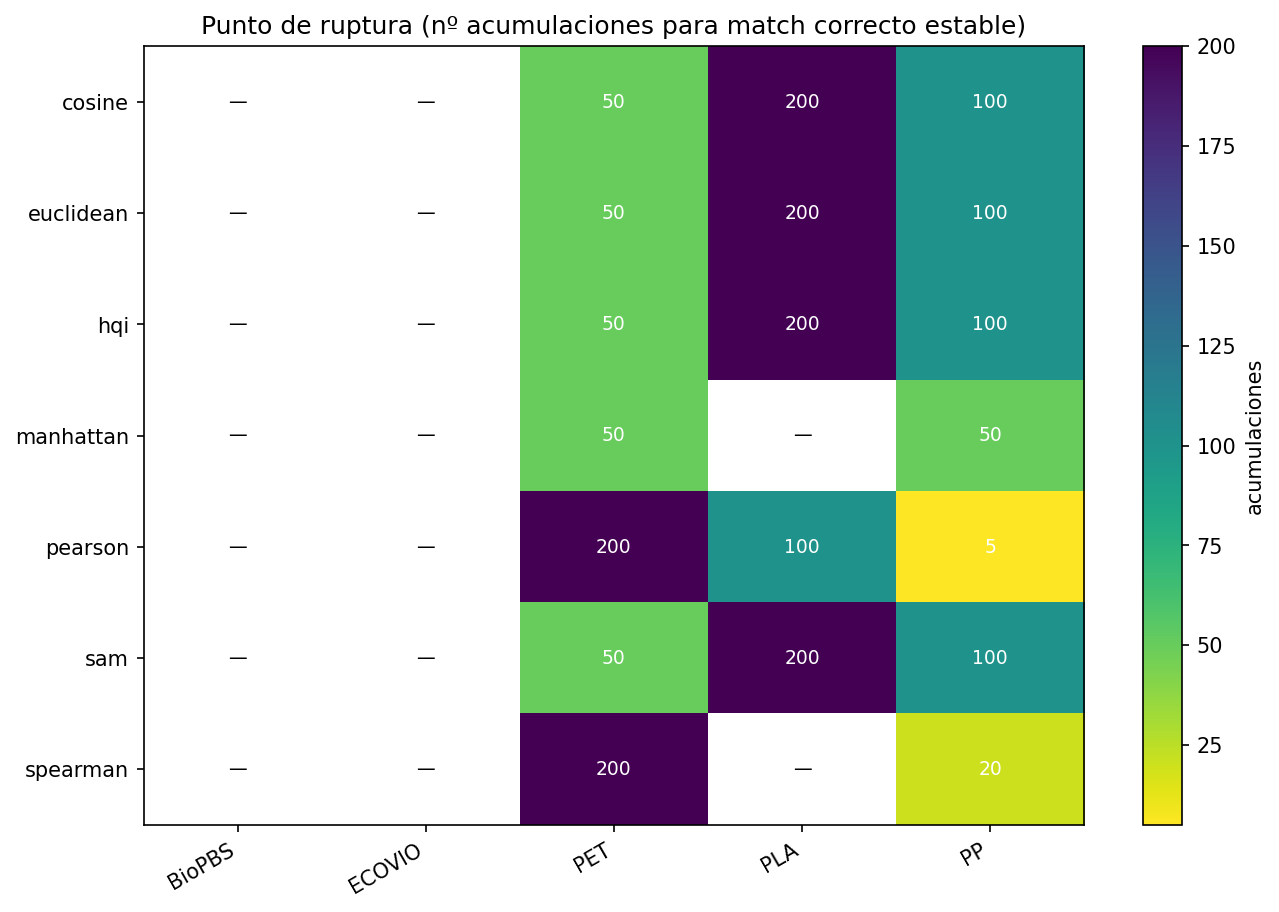
\includegraphics[width=0.85\textwidth]{imagenes/accumulation_breakpoint_heatmap.png}
\caption{Punto de ruptura por métrica y polímero en el eje de acumulación. Las celdas vacías indican que esa métrica nunca identifica correctamente ese polímero de forma estable.}
\label{fig:heatmap-acumulacion}
\end{figure}

Esta tabla exige una lectura cuidadosa, porque el punto de ruptura medio \emph{no} ordena las métricas por calidad. Manhattan presenta el mejor valor aparente (50 acumulaciones), pero ese promedio se calcula únicamente sobre los dos polímeros que llega a identificar (PET y PP); en PLA nunca acierta, mientras que Pearson, con una media peor (101,7), sí resuelve los tres polímeros disponibles. Es decir, la métrica con menor punto de ruptura medio es también una de las de peor exactitud global: el promedio premia implícitamente a quien se rinde en los casos difíciles. Por eso la exactitud de la Tabla~\ref{tab:accuracy} y la columna de polímeros nunca identificados deben leerse junto al punto de ruptura, y no de forma aislada.

\textbf{Comprobación cruzada mediante degradación paramétrica.} Para comprobar si el comportamiento observado depende del mecanismo concreto de pérdida de calidad, se repitió toda la matriz experimental sustituyendo la acumulación real por una degradación sintética (ruido gaussiano a una SNR objetivo, deriva de línea base y submuestreo) aplicada al espectro más limpio de cada polímero. Las Figuras~\ref{fig:similitud-snr} y~\ref{fig:heatmap-degradacion} son las equivalentes de las anteriores con la SNR como eje de calidad.

\begin{figure}[H]
\centering
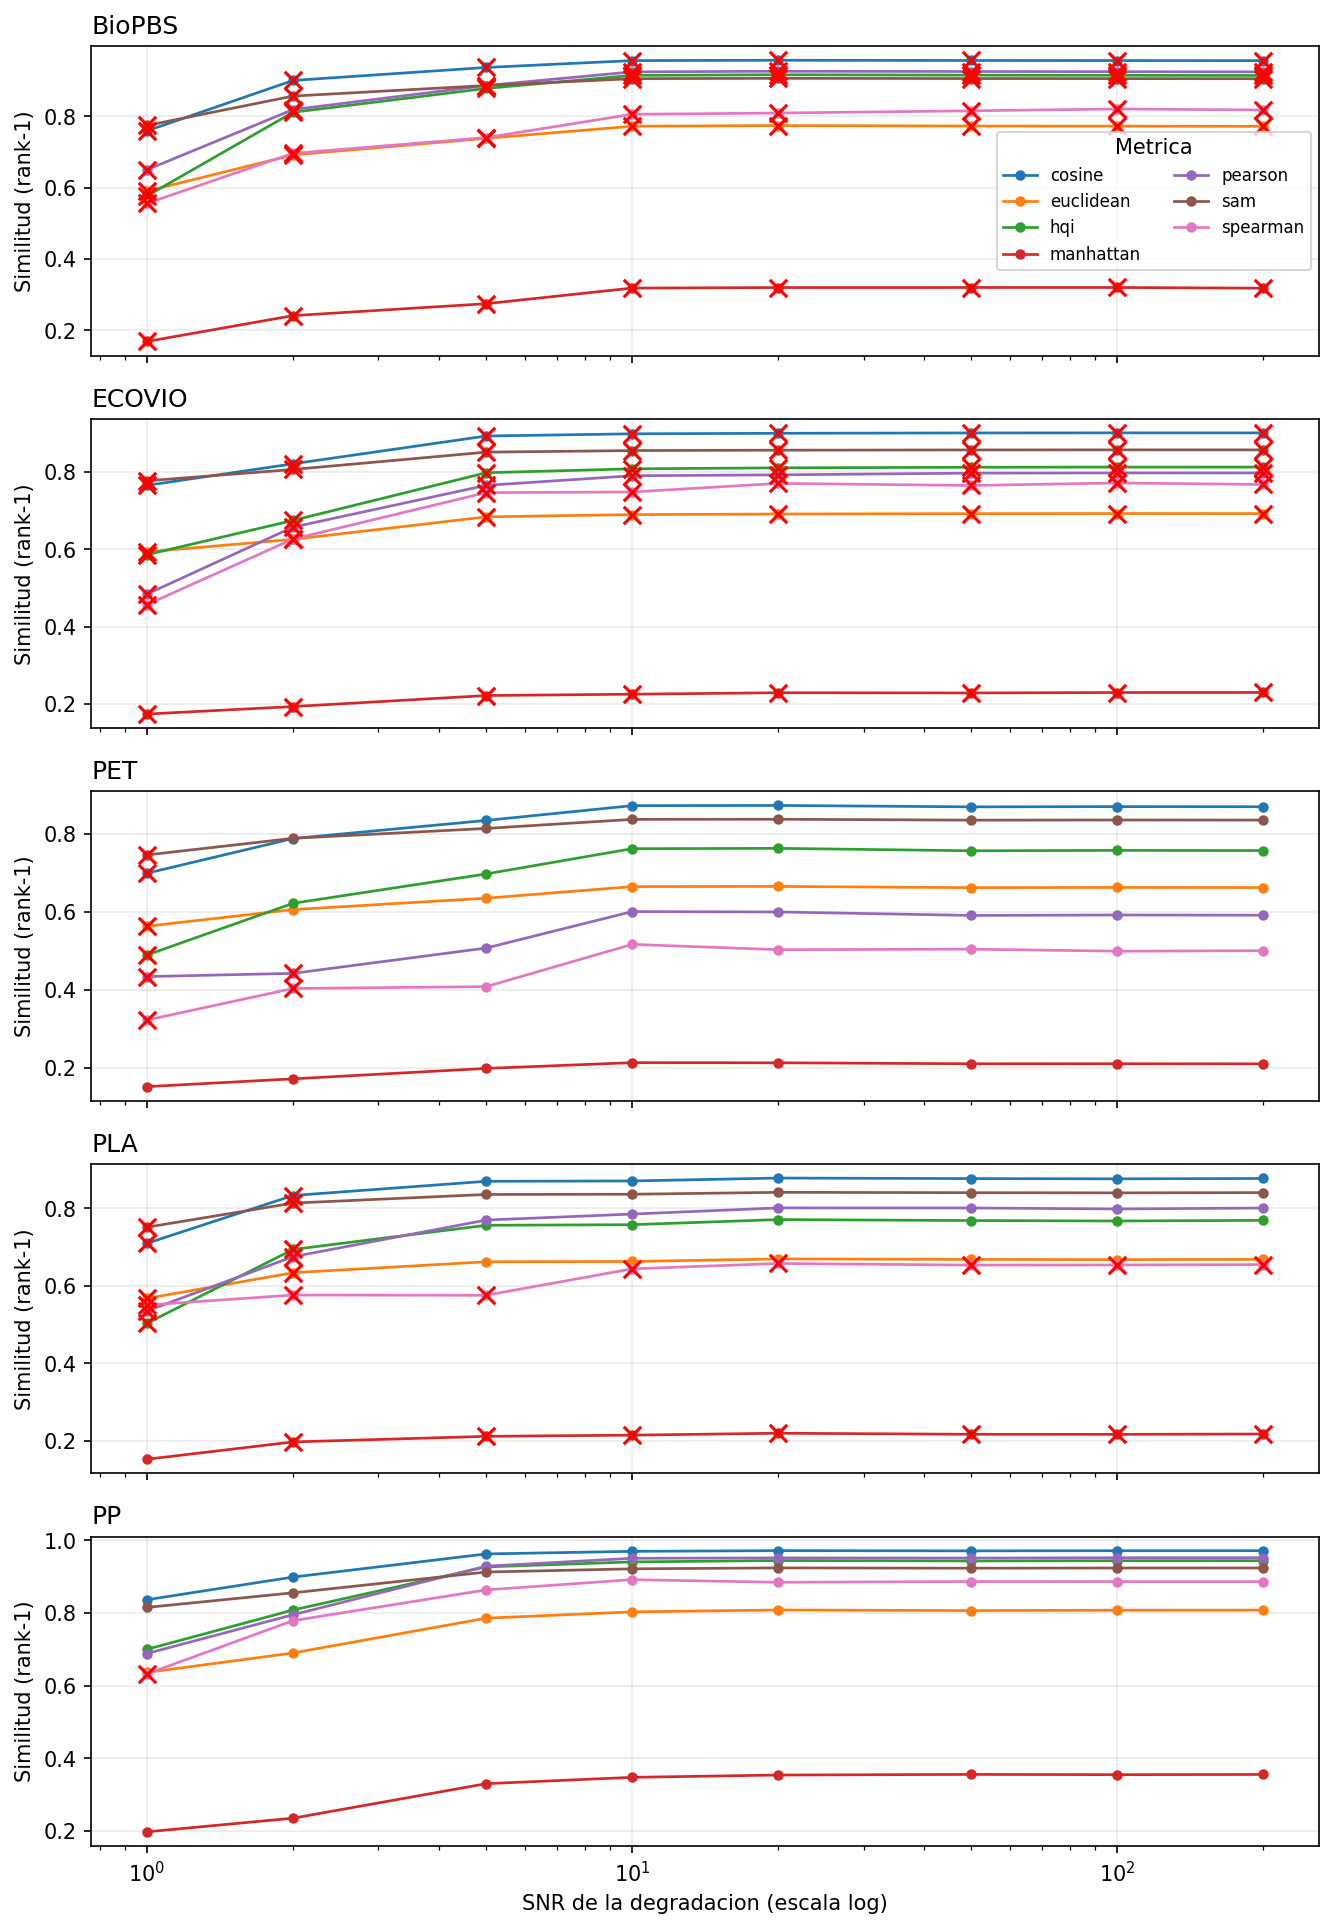
\includegraphics[width=0.85\textwidth]{imagenes/degradation_similarity.png}
\caption{Similitud del mejor resultado (rango~1) frente a la SNR de la degradación paramétrica, una curva por métrica y una subgráfica por polímero medido.}
\label{fig:similitud-snr}
\end{figure}

\begin{figure}[H]
\centering
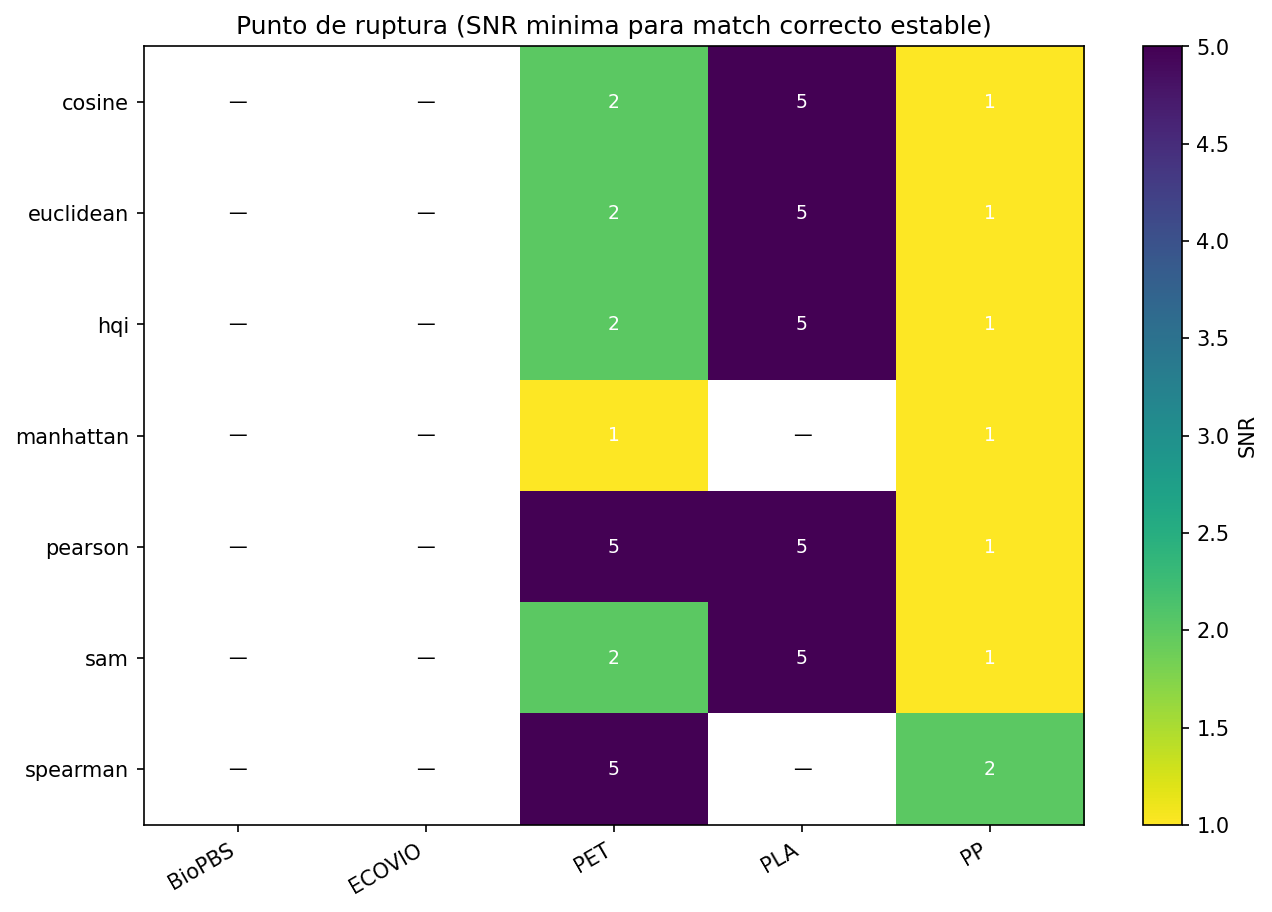
\includegraphics[width=0.85\textwidth]{imagenes/degradation_breakpoint_heatmap.png}
\caption{Punto de ruptura por métrica y polímero en el eje de degradación paramétrica, expresado como SNR mínima para un acierto estable.}
\label{fig:heatmap-degradacion}
\end{figure}

La comparación entre ambos mecanismos arroja una coincidencia parcial: los dos coinciden en que Manhattan y Spearman son las métricas menos fiables, pero discrepan en el primer puesto (Pearson en acumulación real frente al grupo coseno/euclídea/HQI/SAM en degradación paramétrica). Las curvas de la Figura~\ref{fig:similitud-snr} son además más suaves y monótonas que las de la Figura~\ref{fig:similitud-acumulacion}. Tiene sentido: la degradación sintética solo modela la pérdida de relación señal-ruido, mientras que la acumulación real de espectros de integración corta arrastra también artefactos residuales de línea base y de eliminación de picos espurios. Esta diferencia se discute en el Capítulo~5.

\textbf{Hallazgo no anticipado:} dos de los cinco polímeros medidos (BioPBS y ECOVIO) obtienen una exactitud del 0\% con las siete métricas, en todos los niveles de calidad, incluido el de máxima calidad. La causa, verificada, no es una limitación del \textit{pipeline} ni de las métricas: la \emph{Hagelskjær Microplastic Solution Library~1.1} no incluye BioPBS ni ECOVIO en su catálogo de 28~polímeros y 2~minerales de referencia. Esta limitación de cobertura de la base de datos se documenta en el capítulo de Discusión y se propone como línea de trabajo futuro ampliar o combinar la base de datos de referencia para cubrir ambos polímeros.

Estos resultados se amplían en el capítulo de Discusión y se cierran en el depósito final; los números ya proceden de la ejecución real.
